\documentclass[12pt,a4paper,onecolumn]{article}
\usepackage{paralist}
\usepackage{indentfirst}
\usepackage[numbers,sort&compress]{natbib}
\usepackage[left=1.5cm,right=1.5cm,top=1.5cm,bottom=1.5cm]{geometry} %页边距包
\usepackage{amsmath}
\usepackage{flushend,cuted}
\usepackage{caption}
\usepackage{subcaption}
\usepackage{ctex}
\usepackage{pifont}
\usepackage{hyperref}
\usepackage{float} %控制图像固定
\renewcommand\refname{参考文献}
\newcommand{\upcite}[1]{\textsuperscript{\textsuperscript{\cite{#1}}}}
\linespread{1.5}
\hypersetup{
  colorlinks,
  linkcolor=green,
  urlcolor=blue
}
\setCJKfamilyfont{zhsong}{SimSun}
\newcommand{\fs}{\CJKfamily{zhfs}}

\title{\bfseries 分析1988年到2008年间的美国航班延误情况}
\date{}
\author{陈子萌、黎思言、闫施、尹航}

\begin{document}
\captionsetup[figure]{name={图}}
\captionsetup[table]{name={表}}
\maketitle

\begin{abstract}
本文使用了1998年到2008年的每月起飞航班总数、每年起飞航班总数、每月延误航班总数、每年延误航班总数、每月延误航班延误平均时间等数据。基于这些数据,我们整体分析了航班的延误情况。然后我们统计了1998年到2008年的每年每个机场的起飞航班总数、起飞延误航班总数、机场所在城市和机场所在州等数据。基于这些数据,我们分州和城市分析了航班的延误情况。我们统计了美国各州拥有的机场数、总共起降的航班数、取消航班比例、出发延迟超过10分钟的航班比例,到达延迟超过10分钟的航班比例等指标,对美国52个州进行了聚类分析。最后我们统计了纽约肯尼迪机场20年来的每天航班起飞总数、起飞延误总数、降落飞机总数、降落延误航班总数和天气信息等字段。基于这些数据,我们使用随机森林分析天气数据对延误率的影响。
\end{abstract}

\section{数据和方法}

本文使用的了从1988年到2008年的飞机航班数据和纽约肯尼迪机场1998年到2008年的的天气数据。本文从数据库中下载了所有的飞机航班数据和所有的天气数据,然后将数据导入了本地数据库。在本地数据库中统计了1998年到2008年的每月起飞航班总数、每年起飞航班总数、每月延误航班总数、每年延误航班总数、每月延误航班延误平均时间等数据。基于这些数据,我们整体分析了航班的延误情况。在本地数据库中统计了1998年到2008年的每年每个机场的起飞航班总数、起飞延误航班总数、机场所在城市和机场所在州等数据。基于这些数据,我们分州和城市分析了航班的延误情况。在本地数据库中,我们统计了美国各州拥有的机场数、总共起降的航班数、取消航班比例、出发延迟超过10分钟的航班比例,到达延迟超过10分钟的航班比例等指标,对美国52个州进行了聚类分析。在本地数据库中统计了纽约肯尼迪机场20年来的每天航班起飞总数、起飞延误总数、降落飞机总数、降落延误航班总数和天气信息等字段。基于这些数据,我们使用随机森林分析天气数据对延误率的影响。

\section{结果}

\subsection{整体航班延误情况}

\begin{figure}[H]
	\centering
	\includegraphics[width=400pt]{图1.pdf}
	\caption{分年度整体分析}
  \label{图1}
\end{figure}

20年来,美国航班的延迟航班数、总航班数、延迟率和平均延迟时间如图 \ref{图1} 所示。延迟航班是指,航班的实际出发时间比计划的出发时间晚。延迟率是指,延迟航班总数和总航班数的比值。平均延迟时间是指,所有延迟航班的平均延迟时间,单位是分钟。从图中得出以下结论:

(1)20年来,航班总数和延迟航班数的整体趋势是上升的。

(2)20年来,延迟率整体趋势是下降的。上世纪90年代,每年有大于50\%的航班出现延误。但是在2000年之后,延误率降低到45\%以下,在2003年之后稍有波动。

(3)虽然延迟率有显著的下降,但平均延迟时间却上升了。上世纪90年代,平均延迟时间在25分钟以下,2000年以后,平均延迟时间不断上升,目前已经超过了30分钟。

\begin{figure}[H]
	\centering
	\includegraphics[width=400pt]{图2.pdf}
	\caption{分月份整体分析}
	\label{图2}
\end{figure}

每个月的延迟航班数、总航班数、延迟率和平均延迟时间如图 \ref{图2} 所示。从图中得出以下结论:

(1)12月、1月、6月、7月、8月的航班总数和延迟航班数都比其他时间高。说明这段时间是乘坐飞机出行的高峰时期。

(2)在上述的高峰月份,延迟率都大于其他月份。

(3)在上述的高峰月份,延迟时间都大于其他月份。

\subsection{各州航班延误情况}

\begin{figure}[H]
	\centering
	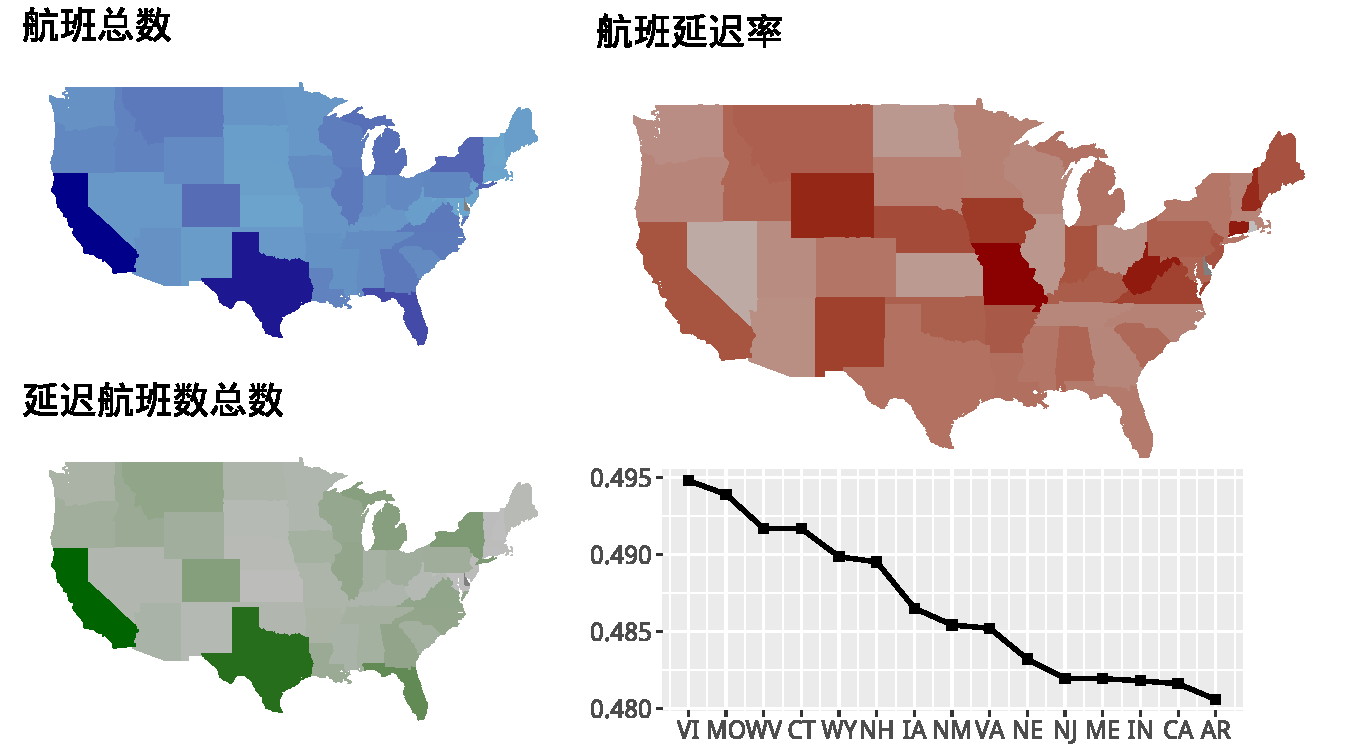
\includegraphics[width=400pt]{图3_2008地图.pdf}
	\caption{各州航班延误情况分析}
     \label{图3_2008地图}
\end{figure}

使用2008年的航班数据,统计了每个州的航班情况如图 \ref{图3_2008地图} 所示。左上角颜色越深表示航班数量越多,左下角颜色越深表示延迟航班数量越多,右上颜色越深表示航班延迟率越高。右下标注出了延迟率最高的15个州。从图中得到以下结论:

(1)航班总数和延迟航班总数最高的州是加利福尼亚州和得克萨斯州。加利福尼亚州是美国本土面积第二大州,人口第一大州和国内生产总值第一大州。德克萨市州是美国本土面积最大州,人口第二大州和国内生产总值第二大州。

(2)美国中部各州航班总数和延迟航班数不高,但航班延迟率相对较高。

(3)航班延迟率最高的15个州为:佛蒙特州、密苏里州、西弗吉尼亚州、康涅狄格州、怀俄明州、新罕布什尔州、爱荷华州、新墨西哥州、弗吉尼亚州、内布拉斯加州、新泽西州、缅因州、印第安纳州、加利福尼亚州、阿肯色州。这些州大部分位于美国中西部地区。

\subsection{主要城市航班情况}

\begin{figure}[H]
	\centering
	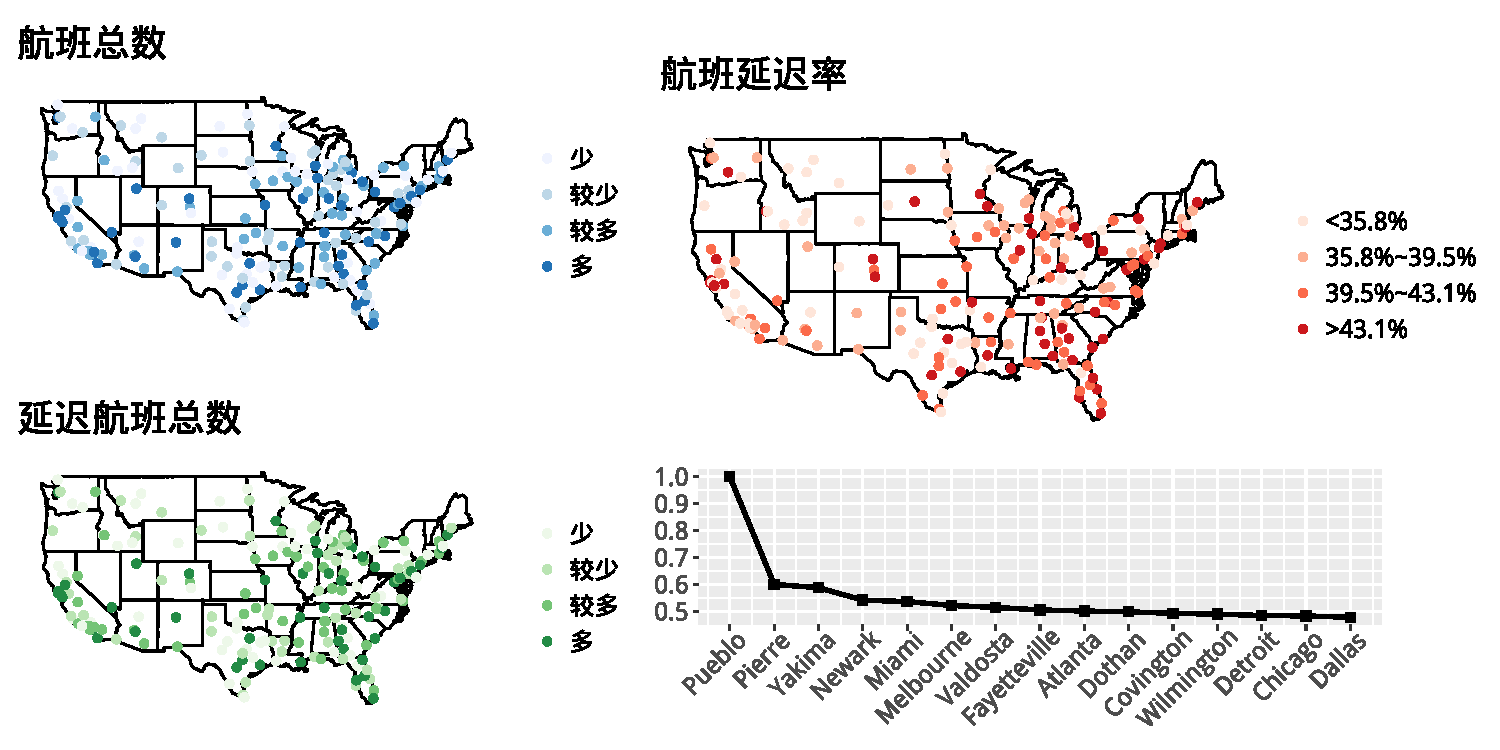
\includegraphics[width=400pt]{图4_2008地图.pdf}
	\caption{主要城市航班情况}
  \label{图4_2008地图}
\end{figure}

使用2008年的航班数据,统计了美国主要城市的航班情况如图 \ref{图4_2008地图} 所示。左上角颜色越深表示航班数量越多,左下角颜色越深表示延迟航班数量越多,右上颜色越深表示航班延迟率越高。右下标注出了延迟率最高的15个州。从图中得到以下结论:

(1)美国东部城市、五大湖周围城市和西海岸加利福尼亚州城市群的航班数量和延迟航班数量较多。

(2)航班延迟率较高的城市集中在美国东部和中部。

\subsection{使用机场信息聚类分析美国各州情况}

我们统计了美国各州拥有的机场数、总共起降的航班数、取消航班比例、出发延迟超过10分钟的航班比例,到达延迟超过10分钟的航班比例等指标,对美国52个州进行了聚类分析。聚类方法使用的是K均值聚类法,迭代次数为20次,为了确定适合的分类个数K,把K可能的取值范围设定到2-7,分别计算K的各个取值下的轮廓系数以及组间方差和总方差之比值,对K在各取值的情况下K均值聚类的效果作出评价。

\begin{table}[H]
	\centering
	\caption{k均值聚类分析}
	\begin{tabular}{ccc}
		\hline
		  k的取值 & 组间方差 & 轮廓系数  \\\hline
	     2 & 0.51776 & 0.7651  \\
		   3 & 0.64168 & 0.2602   \\
       4 & 0.71223 & 0.2656   \\
       5 & 0.76510 & 0.2694   \\
       6 & 0.79325 & 0.2626   \\
       7 & 0.80487 & 0.2606   \\\hline
	\end{tabular}
	\label{k均值}
\end{table}

由表 \ref{k均值} 可知,当K的取值从2变为3时,轮廓系数剧减,因此,首先判断K的最优取值为2。但是,当K=2时,根据聚类结果可得,两类中机场数分别为2个和51个,也就是说,绝大多数机场都被分为一类了,并不能够达到分类的目的,因此,再次观察表格,发现当K=5时轮廓系数达到了最大,而组间方差/总方差在这之后随K取值增加的提升幅度也很小了,因此,把K=5作为比较理想的K取值。当K取5时,组间方差与总方差的比值为76.6\%,所有的地区被分为5个类,每一类中的地区数分别为18,8,12,13,2.

\begin{figure}[H]
	\centering
	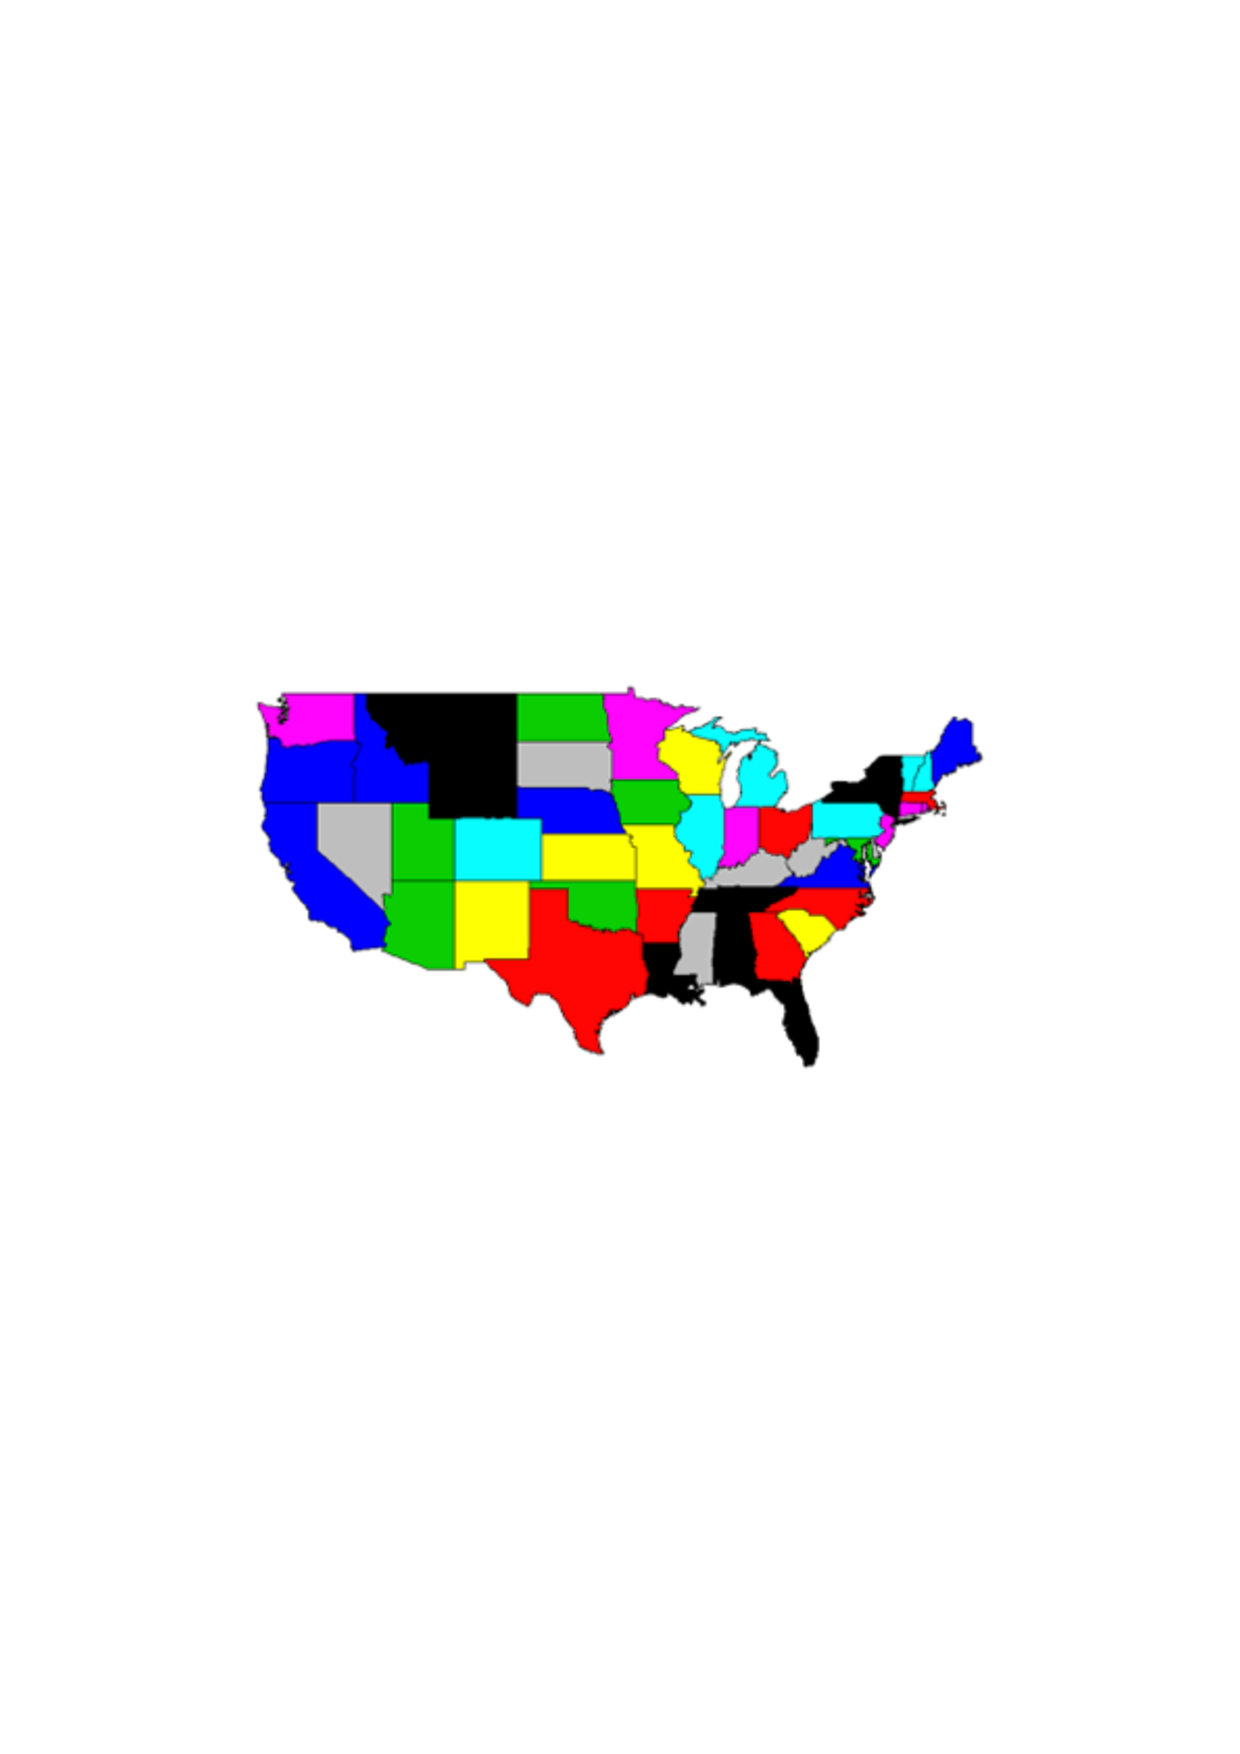
\includegraphics[width=400pt]{聚类分析.pdf}
	\caption{聚类分析结果}
  \label{聚类分析}
\end{figure}

聚类的结果如图 \ref{聚类分析} 所示。类别1的地区特点为拥有最多的机场数量和总起降航班数,取消航班的比例也是最低的;类别2的地区,拥有的机场数量较少,取消航班的比例与降落延迟航班的比例也很低;类别3的地区拥有的机场数量较少,取消航班的比例较低,还拥有最高的起飞延迟比例和最低的降落延迟比例,类别4的地区则拥有最少的机场数,最低的总起降航班数,最高的取消航班比例和降落延迟航班比例,以及最低的起飞延迟比例;类别5的地区拥有的机场数量较多,取消航班的比例也较高。

\subsection{使用天气信息预测肯尼迪机场的航班延误率}

由上文可知,美国航线的延误情况不容乐观。动辄40\%~50\%的延误率不仅影响了人们的出行,更对美国的航空运输行业产生了负面的影响。航空延误的现象出现的原因多种多样,天气原因是造成航空延误的主要原因之一。出发地机场天气状况不宜起飞;目的地机场天气状况不宜降落;飞行航路上气象状况不宜飞越等等都可能导致航空延误。本文主要研究出发地天气状况不宜起飞或者目的地天气状况不宜降落导致的延误。

本文选取的研究对象是纽约约翰·菲茨杰拉德·肯尼迪国际机场。该机场是纽约市的主要国际机场,是全世界最大机场之一。机场于1942年始建,1948年7月1日首次有商业航班,并于7月31日正式命名为“纽约国际机场”。1963年11月22日美国总统约翰·肯尼迪遇刺身亡,12月24日机场改名为“约翰·菲茨杰拉德·肯尼迪国际机场”以纪念这位先总统;随后,机场的国际航空运输协会机场代码更新为JFK。肯尼迪国际机场设有9个客运航站楼,各航站以U形格局围绕机场中心区域的停车场、酒店、供电设施等设施。AirTrain和道路均接驳各个航站。JFK占地4,930英亩,其中包括中央航站区的880英亩。约37,000人在JFK工作。机场为纽约 - 新泽西州大都市区贡献约373亿美元的产值,同时创造了约256,000个工作机会,提供了134亿美元的薪资。JFK还是世界领先的国际航空货运中心之一。机场提供面积近400万平方英尺的的货物仓库和办公空间。整个航空货运区都被指定为外贸区。 JFK通过长距离、直达和不间断的空运,为世界主要的航空货运市场服务。在本文中,我们使用肯尼迪机场的数据分析天气对肯尼迪机场的航班延误率的影响。

\subsubsection{描述统计}

\begin{figure}[H]
	\centering
	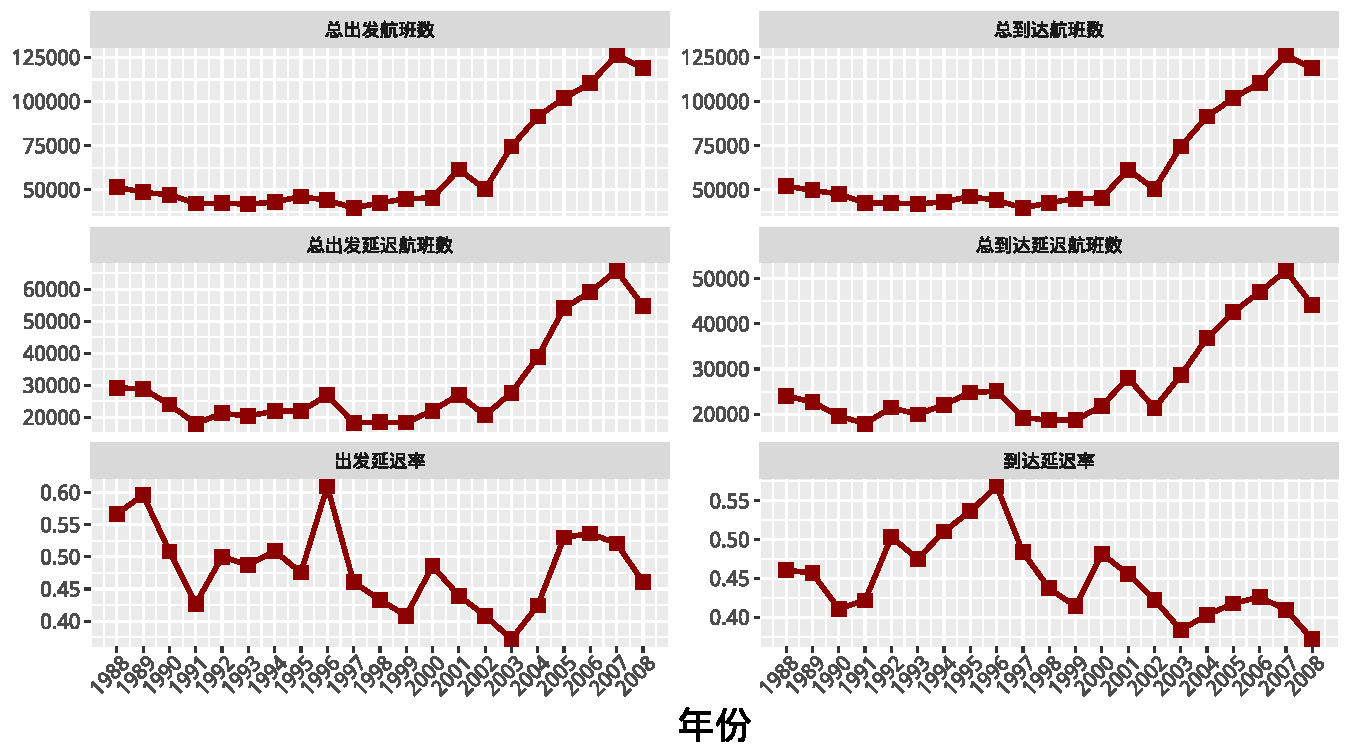
\includegraphics[width=400pt]{图5_肯尼迪机场描述统计.pdf}
	\caption{肯尼迪机场基本情况}
  \label{图5_肯尼迪机场描述统计}
\end{figure}

纽约肯尼迪机场20年来的起飞航班和降落航班的基本情况如图 \ref{图5_肯尼迪机场描述统计} 从图中可以得出以下结论:

(1)2000年以来,肯尼迪机场起飞的航班和到达的国内航班数量都显著增加。从一年5万趟国内航班的水平上升到一年12.5万趟国内航班。增长了约1.5倍。

(2)2000年以来,肯尼迪机场出发的延迟航班和到达的延迟航班数量都显著上升。从一年2万班延迟航班的水平上升到一年约5.5万班。

(3)肯尼迪机场的出发航班和到达航班的延迟率都呈现出先上升后下降的变化趋势。

\subsubsection{使用天气信息预测起飞航班的延误率}

本文使用1988年到2008年每天纽约肯尼迪机场的天气信息预测从肯尼迪机场起飞的航班的延误率。

本文选取的自变量特征有。"Year":年;"Month":月  ;"DayofMonth":日;"Maxtemp":最高温度;"Meantemp":平均温度;"Mintemp":最低温度;"Maxdewpoint":最高露点温度;"Meandewpoint":平均露点温度;"Mindewpoint":最低露点温度;"Maxhumidity":最高湿度;"Meanhumidity":平均湿度;"Minhumidity":最低湿度;"Maxsealevelpre":平均海拔高度:"Meansealevelpre";最低海拔高度:"Minsealevelpre";最高能见度:"Maxvisibility";平均能见度:"Meanvisibility";最低能见度:"Minvisibility";最高风速:"Maxwindspeed";最低风速:"Meanwindspeed";降水量:"Rainfall";云量:"Cloudcover";天气状况:"Events";风向度数:"Winddirdegrees"等24个自变量。因变量是起飞航班的延误率,本文将起飞航班延误率小于50\%的天分为一组,将起飞航班延误率大于50\%的天分为另一组。

自变量中的缺失数据的处理办法如下,最高温度、最低温度和平均温度中的缺失数据删除,一共删除了460条缺失数据。最高能见度、最低能见度和平均能见度中有12个缺失数据,采用中位数插补。风向度数中有7个缺失数据,采用中位数插补。天气状况中的空缺数据,采用“orther”水平补齐。处理完毕后,一共有7208个有效数据。在延误率较低的组中有4026个数据,在延误率较高的组中有3182个数据。

本文将上述数据按照75\%的训练集和25\%的测试集进行划分,对训练集样本建立了300棵CART分类树的随机森林模型。输出预测结果和自变量的重要程度。重要程度如图 \ref{起飞模型1imp} 。预测准确率如表 \ref{起飞模型1}。可见预测准确率为75.42\%. 在延误率较低的组中,预测准确率是79.1\%. 在延误率较高的组中,预测准确率是70.75\%.对飞机起飞延误影响最大的天气因素是天气状况,其次是最低能见度。

\begin{figure}[H]
	\centering
	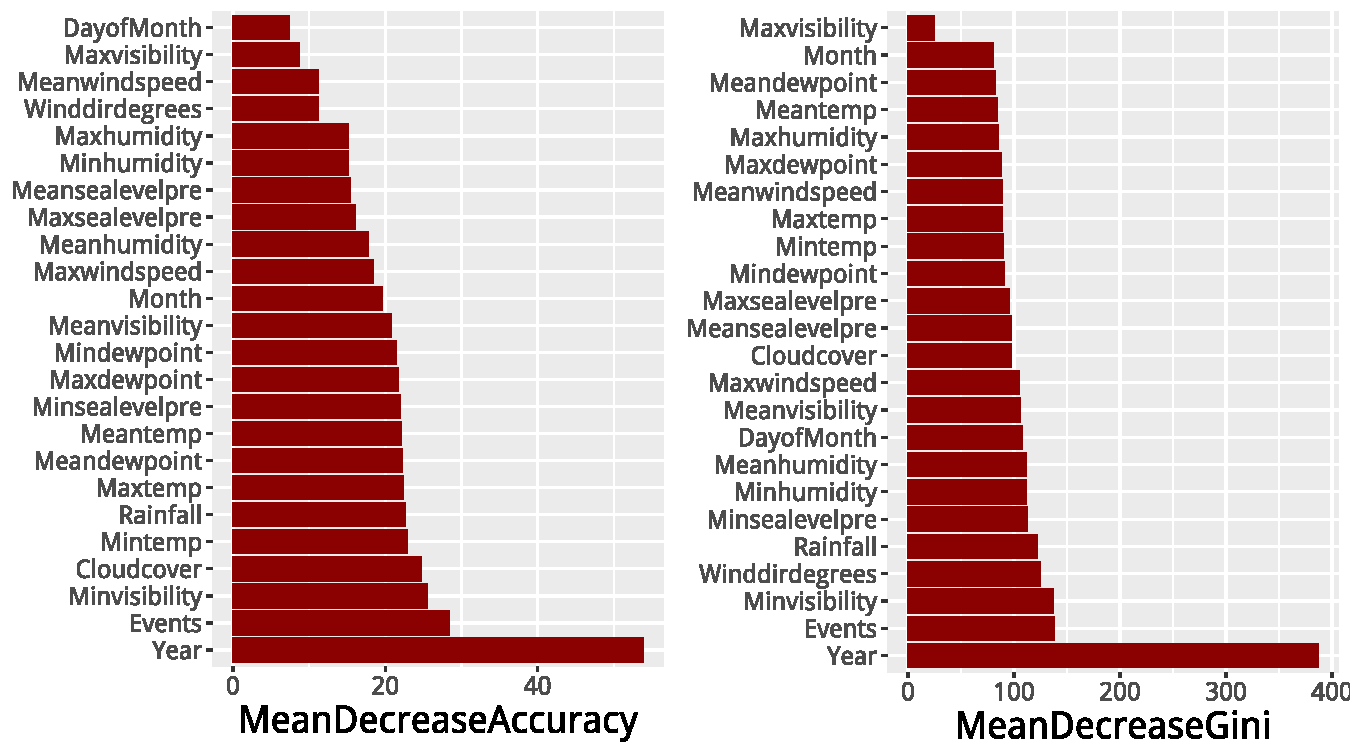
\includegraphics[width=400pt]{起飞模型1imp.pdf}
	\caption{使用天气信息预测起飞航班的延误率的变量重要性}
  \label{起飞模型1imp}
\end{figure}

\begin{table}[H]
	\centering
	\caption{使用天气信息预测起飞航班的延误率的预测混淆矩阵}
	\begin{tabular}{ccc}
		\hline
		   &  (0,0.5]  & (0.5,1]  \\
	     (0,0.5] & 788 & 207   \\
		 (0.5,1] & 236 & 571   \\\hline
	\end{tabular}
	\label{起飞模型1}
\end{table}

\subsubsection{使用天气信息预测降落航班的延误率}

降落航班的自变量和因变量选取过程和缺失值处理过程和起飞航班的处理过程类似。在延误率较低的租中有4888个数据,在延误率较高的组中有2320个数据。本文依旧划分75\%的训练集和25\%的测试集,使用300棵分类树的随机森林模型估计降落航班的延误率。输出预测结果和自变量的重要程度。重要程度如图 \ref{到达模型1imp} 。预测准确率如表 \ref{到达模型1}。可见预测准确率为78.02\%.

\begin{figure}[H]
	\centering
	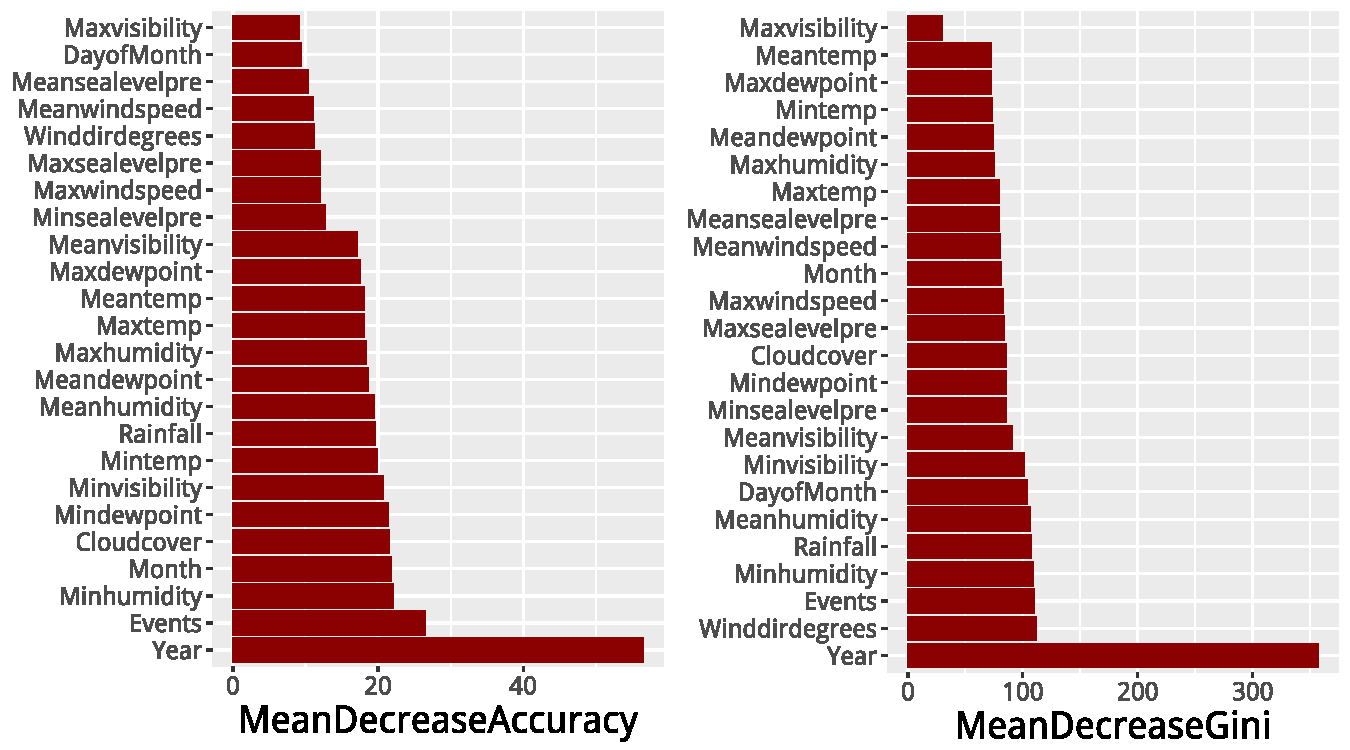
\includegraphics[width=400pt]{到达模型1imp.pdf}
	\caption{使用天气信息预测降落航班的延误率的变量重要性}
  \label{到达模型1imp}
\end{figure}

\begin{table}[H]
	\centering
	\caption{使用天气信息预测降落航班的延误率的预测混淆矩阵}
	\begin{tabular}{ccc}
		\hline
		     &  (0,0.5]  & (0.5,1]  \\
	     (0,0.5] & 1078 & 123   \\
		 (0.5,1] & 273 & 328   \\\hline
	\end{tabular}
	\label{到达模型1}
\end{table}

从图 \ref{到达模型1imp} 中可知,对飞机降落延误影响最大的天气因素有:天气状况、最低湿度、云量等。从预测效果看来,对延误率较小的组的预测效果较好,但是对延误率较大组的预测效果不好。

这是因为,在降落航班中,延误率较高的数据和延误率较低的数据个数并不平衡。对于不平衡数据一般采用对少数组过抽样或对多数组欠抽样的方法提高对少数组的预测精度。本文采用过抽样的方法解决不平衡数据的分类问题,本文采取的不平衡数据处理方法是对少数组过抽样的方法。我们在训练集中对少数组过抽样了1000个样本。过抽样之后的预测结果和变量重要程度如图 \ref{到达模型11imp} 和表 \ref{到达模型11}。

\begin{figure}[H]
	\centering
	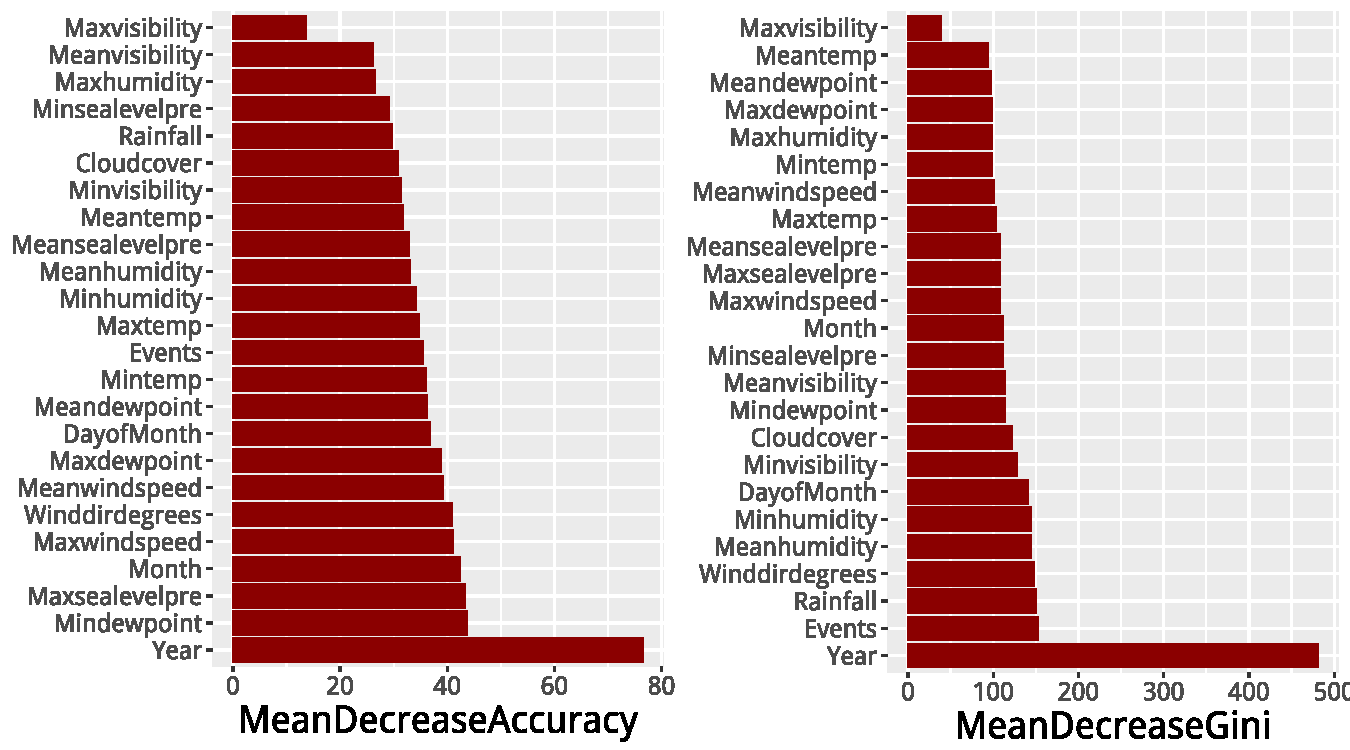
\includegraphics[width=400pt]{到达模型11imp.pdf}
	\caption{使用天气信息预测降落航班的延误率的变量重要性2}
	\label{到达模型11imp}
\end{figure}

\begin{table}[H]
	\centering
	\caption{使用天气信息预测降落航班的延误率的预测混淆矩阵2}
	\begin{tabular}{ccc}
		\hline
		    &  (0,0.5]  & (0.5,1]  \\
	     (0,0.5] & 1035 & 166  \\
		 (0.5,1] & 234 & 367   \\\hline
	\end{tabular}
	\label{到达模型11}
\end{table}

从图 \ref{到达模型11imp} 中可知,对飞机降落延误影响最大的天气因素有最低露点温度、最高海平面高度、最高风速等。预测准确率为77.80\%.总体预测准确率下降了,但是对于少数组的预测准确率上升了。准确率从57.58\%上升到61.06\%.

\end{document}
